\documentclass[11pt,a4paper]{article}
\usepackage[utf8]{inputenc}
\usepackage[english]{babel}
\usepackage{amsmath}
\usepackage{amsfonts}
\usepackage{amssymb}
\usepackage{graphicx}
\usepackage{hyperref}
\usepackage{listings}
\usepackage{xcolor}
\usepackage{geometry}
\usepackage{fancyhdr}
\usepackage{caption}
\usepackage{subcaption}
\usepackage{booktabs}
\usepackage{float}
\usepackage{enumitem}

% Page geometry
\geometry{margin=1in}

% Code listing style
\lstset{
    basicstyle=\ttfamily\small,
    keywordstyle=\color{blue},
    commentstyle=\color{gray},
    stringstyle=\color{red},
    showstringspaces=false,
    breaklines=true,
    frame=single,
    numbers=left,
    numberstyle=\tiny\color{gray}
}

% Hyperlink colors
\hypersetup{
    colorlinks=true,
    linkcolor=blue,
    filecolor=magenta,
    urlcolor=cyan,
    citecolor=blue
}

\title{\textbf{Pipelined Reliable Transfer Protocol:\\Design \& Analysis Report}}
\author{Computer Networks\\Mini-Project 2 - Custom Reliable Transport Protocol}
\date{November 22, 2025}

\begin{document}

\maketitle
\thispagestyle{empty}

\begin{abstract}
This report presents the design, implementation, and analysis of a custom \textbf{Pipelined Reliable Transfer Protocol} that provides connection-oriented, reliable data transfer with flow control and congestion control mechanisms. The protocol is implemented in Python using UDP sockets as the unreliable transport layer and includes a simulation framework for testing under controlled network conditions with packet loss and bit errors. 

    \textbf{Key features} include TCP Reno-style congestion control, sliding window flow control, pipelined transmission, and comprehensive testing with traffic analysis. The protocol successfully passes all functional tests with 100\% data integrity (10,000/10,000 bytes delivered) despite 10\% configured packet loss using only a single retransmission in 15.30 seconds. Performance testing demonstrates 92,160 bytes of application data transferred (103,396 total bytes including 20-byte headers per packet), 8.31 KB/s throughput, and 8.91\% actual packet loss over 12.16 seconds with robust congestion control adaptation (final cwnd: 3.24 packets, ssthresh: 2.0 packets). Fairness testing demonstrates near-perfect bandwidth sharing with Jain's Fairness Index of 0.998 between two competing flows, proving TCP-friendliness.
\end{abstract}

\newpage
\tableofcontents
\newpage

\section{Protocol Specification}

\subsection{Protocol Overview}

Our protocol operates above the UDP layer, providing TCP-like reliability and flow control while using unreliable datagrams for transport. The protocol is designed to be:

\begin{itemize}
    \item \textbf{Connection-oriented}: Establishes explicit connections using handshakes
    \item \textbf{Reliable}: Guarantees in-order, error-free delivery
    \item \textbf{Pipelined}: Multiple packets in flight for efficiency
    \item \textbf{Flow-controlled}: Respects receiver's buffer capacity
    \item \textbf{Congestion-aware}: Adapts to network conditions
\end{itemize}

\subsection{Packet Format}

Each packet consists of a 20-byte fixed header followed by a variable-length payload. The header uses big-endian byte order. The packet structure is shown below:

\begin{verbatim}
0                   1                   2                   3
0 1 2 3 4 5 6 7 8 9 0 1 2 3 4 5 6 7 8 9 0 1 2 3 4 5 6 7 8 9 0 1
+-+-+-+-+-+-+-+-+-+-+-+-+-+-+-+-+-+-+-+-+-+-+-+-+-+-+-+-+-+-+-+-+
|           Checksum            |      Sequence Number (high)   |
+-+-+-+-+-+-+-+-+-+-+-+-+-+-+-+-+-+-+-+-+-+-+-+-+-+-+-+-+-+-+-+-+
|                  Sequence Number (low)                        |
+-+-+-+-+-+-+-+-+-+-+-+-+-+-+-+-+-+-+-+-+-+-+-+-+-+-+-+-+-+-+-+-+
|                      Acknowledgment Number                    |
+-+-+-+-+-+-+-+-+-+-+-+-+-+-+-+-+-+-+-+-+-+-+-+-+-+-+-+-+-+-+-+-+
|                         Packet Type                           |
+-+-+-+-+-+-+-+-+-+-+-+-+-+-+-+-+-+-+-+-+-+-+-+-+-+-+-+-+-+-+-+-+
|                      Receiver Window (rwnd)                   |
+-+-+-+-+-+-+-+-+-+-+-+-+-+-+-+-+-+-+-+-+-+-+-+-+-+-+-+-+-+-+-+-+
|        Data Length (H)        |   Data (variable length)...   |
+-+-+-+-+-+-+-+-+-+-+-+-+-+-+-+-+-+-+-+-+-+-+-+-+-+-+-+-+-+-+-+-+
\end{verbatim}

\textbf{Header Fields (20 bytes total):}
\begin{itemize}
    \item \textbf{Checksum (16 bits, offset 0-1)}: 16-bit one's complement checksum for error detection
    \item \textbf{Sequence Number (32 bits, offset 2-5)}: Packet-based sequence number for ordering
    \item \textbf{Acknowledgment Number (32 bits, offset 6-9)}: Next expected packet sequence number (cumulative ACK)
    \item \textbf{Packet Type (32 bits, offset 10-13)}: Packet type enum (SYN=0, SYN\_ACK=1, ACK=2, DATA=3, FIN=4, FIN\_ACK=5)
    \item \textbf{Receiver Window (32 bits, offset 14-17)}: Available buffer space at receiver in number of packets (flow control)
    \item \textbf{Data Length (16 bits, offset 18-19)}: Length of data payload in bytes
\end{itemize}

\textbf{Encoding:} Big-endian byte order (network byte order) using struct format \texttt{!IIIIH}

\subsection{Packet Types}

\begin{table}[H]
\centering
\begin{tabular}{@{}lll@{}}
\toprule
\textbf{Type} & \textbf{Value} & \textbf{Description} \\ \midrule
SYN & 0 & Connection establishment request \\
SYN\_ACK & 1 & Connection acknowledgment \\
ACK & 2 & Acknowledgment packet \\
DATA & 3 & Data packet \\
FIN & 4 & Connection termination request \\
FIN\_ACK & 5 & Termination acknowledgment \\ \bottomrule
\end{tabular}
\caption{Packet Types}
\end{table}

\subsection{Connection Management}

\subsubsection{Connection Establishment (3-Way Handshake)}

The connection establishment follows the standard TCP 3-way handshake:

\begin{enumerate}
    \item Client sends SYN with initial sequence number
    \item Server responds with SYN-ACK containing its sequence number and acknowledgment
    \item Client sends ACK to confirm connection
    \item Connection enters ESTABLISHED state
\end{enumerate}

\subsubsection{Connection Termination (2-Way Handshake)}

Connection termination uses a simplified 2-way handshake:

\begin{enumerate}
    \item Client sends FIN packet
    \item Server responds with FIN-ACK packet
    \item Both endpoints enter CLOSED state
\end{enumerate}

\textbf{Note:} Unlike TCP's 4-way termination, our protocol uses a simplified 2-way process. The server's FIN-ACK serves both as an acknowledgment of the client's FIN and the server's own termination signal.

\subsection{Flow Control Mechanism}

Flow control prevents the sender from overwhelming the receiver's buffer using a \textbf{sliding window} approach:

\begin{itemize}
    \item \textbf{Receiver Window (rwnd)}: Advertised by receiver in every packet
    \item \textbf{Effective Window}: $\min(\text{cwnd}, \text{rwnd})$ where is congestion window
    \item \textbf{Sender Constraint}: $(\text{next\_seq\_num} - \text{send\_base}) < \text{effective\_window}$
\end{itemize}

The receiver maintains a buffer for out-of-order packets and updates rwnd based on available space:

\begin{equation}
\text{rwnd (packets)} = \lceil\frac{\max(\text{max\_buffer\_size} - \text{current\_buffer\_usage}, 0)}{\text{MSS}}\rceil
\end{equation}

\subsection{Congestion Control Mechanism}

Our protocol implements \textbf{TCP Reno-style} congestion control with four key states:

\subsubsection{States}

\textbf{1. Slow Start}
\begin{itemize}
    \item Initial $\text{cwnd} = 1$ MSS
    \item Exponential growth: $\text{cwnd} \leftarrow \text{cwnd} + 1$ per ACK
    \item Continues until $\text{cwnd} \geq \text{ssthresh}$ or packet loss
\end{itemize}

\textbf{2. Congestion Avoidance}
\begin{itemize}
    \item Linear growth: $\text{cwnd} \leftarrow \text{cwnd} + \frac{1}{\text{cwnd}}$ per ACK
    \item Conservative increase to avoid congestion
\end{itemize}

\textbf{3. Fast Retransmit}
\begin{itemize}
    \item Triggered by 3 duplicate ACKs
    \item Immediately retransmit lost packet without waiting for timeout
\end{itemize}

\textbf{4. Fast Recovery}
\begin{itemize}
    \item On 3 duplicate ACKs: $\text{ssthresh} = \text{cwnd} / 2$, $\text{cwnd} = \text{ssthresh} + 3$
    \item Linear increase: $\text{cwnd} \leftarrow \text{cwnd} + 1$ per duplicate ACK
    \item Return to congestion avoidance on new ACK
\end{itemize}

\subsubsection{Timeout Event}

On timeout:
\begin{align}
\text{ssthresh} &= \max\left(\frac{\text{cwnd}}{2}, 2\right) \\
\text{cwnd} &= 1 \\
\text{state} &= \text{SLOW\_START}
\end{align}

\subsubsection{Mathematical Model}

Let $W(t)$ be the congestion window at time $t$:

\begin{itemize}
    \item \textbf{Slow Start:} $W(t+1) = W(t) + 1$ (exponential)
    \item \textbf{Congestion Avoidance:} $W(t+1) = W(t) + \frac{1}{W(t)}$ (linear)
    \item \textbf{On Loss:} $W_{\text{new}} = \max\left(\frac{W_{\text{old}}}{2}, 2\right)$
\end{itemize}

\subsection{Reliability Mechanisms}

\subsubsection{Error Detection}
\begin{itemize}
    \item \textbf{Checksum}: 16-bit one's complement checksum computed over entire packet (excluding checksum field itself)
    \item \textbf{Algorithm}: Sum all 16-bit words with wraparound, then take one's complement
    \item \textbf{Validation}: Receiver recomputes checksum and compares with received value; drops corrupted packets
\end{itemize}

\subsubsection{Retransmission}
\begin{itemize}
    \item \textbf{Timeout-based}: Retransmit oldest unacknowledged packet on timeout
    \item \textbf{Fast Retransmit}: Retransmit on 3 duplicate ACKs
\end{itemize}

\subsubsection{Acknowledgments}
\begin{itemize}
    \item \textbf{Cumulative ACKs}: Receiver sends ACK for next expected sequence number
    \item \textbf{Immediate ACKs}: Sent for every received DATA packet
\end{itemize}

\section{Implementation Design}

\subsection{Architecture Overview}

The implementation consists of four main components arranged in layers:

\begin{enumerate}
    \item \textbf{Application Layer}: Uses protocol API for send/receive operations
    \item \textbf{ReliableTransportProtocol}: Connection management, flow control, congestion control, packet buffering
    \item \textbf{UnreliableChannel}: Simulates packet loss, bit errors, and network delay
    \item \textbf{UDP Socket}: Best-effort datagram delivery
\end{enumerate}

\subsection{Key Classes}

\subsubsection{Packet Class}
\begin{itemize}
    \item Encapsulates protocol packet structure
    \item Methods: \texttt{serialize()}, \texttt{deserialize()}, \texttt{\_calculate\_checksum()}
    \item Handles conversion between Python objects and bytes
\end{itemize}

\subsubsection{UnreliableChannel Class}
\begin{itemize}
    \item Simulates network impairments for testing
    \item Configurable loss rate (default: 5\%)
    \item Configurable error rate (default: 1\%)
    \item Simulates variable network delay (1-50ms)
\end{itemize}

\subsubsection{CongestionControl Class}
\begin{itemize}
    \item Implements TCP Reno congestion control
    \item Maintains cwnd, ssthresh, and state
    \item Methods: \texttt{on\_ack\_received()}, \texttt{on\_timeout()}, \texttt{get\_window\_size()}
\end{itemize}

\subsubsection{ReliableTransportProtocol Class}
\begin{itemize}
    \item Main protocol implementation
    \item Connection management (connect, listen, close)
    \item Data transmission (send, receive)
    \item Automatic retransmission and acknowledgment
    \item Statistics collection for analysis
\end{itemize}

\subsection{Threading Model}

The protocol uses a multi-threaded design:

\begin{itemize}
    \item \textbf{Main Thread}: Application-level send/receive operations
    \item \textbf{Receiver Thread}: Continuously listens for incoming packets
    \item \textbf{Timer Thread}: Handles retransmission timeouts
\end{itemize}

\textbf{Synchronization:}
\begin{itemize}
    \item Locks protect shared data structures (send buffer, receive buffer, statistics)
    \item Thread-safe queue operations for packet buffering
\end{itemize}

\subsection{State Machine}

The protocol implements a connection state machine with the following states:

\begin{itemize}
    \item CLOSED: No connection
    \item LISTEN: Waiting for incoming connection
    \item SYN\_SENT: Sent SYN, waiting for SYN-ACK
    \item SYN\_RECEIVED: Received SYN, sent SYN-ACK
    \item ESTABLISHED: Connection active
    \item FIN\_WAIT: Sent FIN, waiting for ACK
    \item CLOSE\_WAIT: Received FIN, ready to close
\end{itemize}

\subsection{Packet Loss Simulation}

\textbf{Challenge:} Testing reliability mechanisms requires packet loss, but local loopback doesn't drop packets.

\textbf{Solution:} Implement \texttt{UnreliableChannel} class that probabilistically drops packets before sending.

\textbf{Benefits:}
\begin{itemize}
    \item Controlled testing environment
    \item Reproducible results with seed
    \item Adjustable impairment levels
    \item No need for network simulator
\end{itemize}

\section{Testing Methodology}

\subsection{Test Suite Overview}

We developed a comprehensive test suite (\texttt{test\_protocol.py}) covering five key areas:

\begin{table}[H]
\centering
\begin{tabular}{@{}llll@{}}
\toprule
\textbf{Test \#} & \textbf{Test Name} & \textbf{Focus} & \textbf{Pass Criteria} \\ \midrule
1 & Connection Establishment & 3-way handshake & Both endpoints ESTABLISHED \\
2 & Reliable Data Transfer & Reliability with loss & All data received correctly \\
3 & Congestion Control & cwnd adaptation & cwnd evolves properly \\
4 & Flow Control & Window limitation & Sender respects rwnd \\
5 & Connection Termination & Clean shutdown & Both endpoints CLOSED \\ \bottomrule
\end{tabular}
\caption{Test Suite Overview}
\end{table}

Additionally, we run an extended \textbf{Performance Test} (10-second continuous transfer) to collect detailed statistics for analysis.

\subsection{Test Configuration}

\textbf{Network Conditions:}
\begin{itemize}
    \item Loss rate: 5-10\% (simulates moderately lossy network)
    \item Error rate: 1-3\% (simulates bit corruption)
    \item Delay: 1-50ms (simulates network latency)
\end{itemize}

\textbf{Protocol Parameters:}
\begin{itemize}
    \item Maximum Segment Size (MSS): 1024 bytes
    \item Initial cwnd: 1 MSS
    \item Initial ssthresh: 64 MSS
    \item Timeout interval: 1 second
    \item Receiver buffer: 64 KB
\end{itemize}

\subsection{Running the Tests}

\textbf{Step 1:} Run the test suite
\begin{lstlisting}[language=bash]
python test_protocol.py
\end{lstlisting}

\textbf{Step 2:} Generate analysis figures
\begin{lstlisting}[language=bash]
python generate_figures.py
\end{lstlisting}

\textbf{Step 3:} Review results
\begin{itemize}
    \item Check console output for test results
    \item Review \texttt{test\_results.json} for raw data
    \item Examine figures in \texttt{figures/} directory
\end{itemize}

\section{Traffic Analysis}

\subsection{Analysis Approach}

We analyze our protocol's behavior through multiple perspectives:

\begin{enumerate}
    \item \textbf{Packet-level Analysis}: Individual packet events (sent, lost, ACKed)
    \item \textbf{Window Evolution}: How cwnd and rwnd change over time
    \item \textbf{Throughput Analysis}: Data transfer rate under various conditions
    \item \textbf{Loss Recovery}: Retransmission patterns and recovery time
\end{enumerate}

\subsection{Instrumentation}

The protocol implementation includes comprehensive statistics collection:

\begin{lstlisting}[language=Python]
stats = {
    'packets_sent': int,           # Total packets sent
    'packets_received': int,       # Total packets received
    'packets_lost': int,           # Packets lost in channel
    'retransmissions': int,        # Retransmitted packets
    'bytes_sent': int,             # Total bytes sent
    'bytes_received': int,         # Total bytes received
    'cwnd_history': [float],       # cwnd over time
    'timestamps': [float],         # Corresponding timestamps
    'throughput_history': [float], # Throughput samples
}
\end{lstlisting}

\subsection{Key Observations}

\subsubsection{Connection Establishment}
\begin{itemize}
    \item \textbf{3-way handshake completes successfully} even with packet loss
    \item Timeout mechanism ensures handshake completion
    \item Connection setup time: $\sim$0.5-1.0 seconds under normal conditions
\end{itemize}

\subsubsection{Reliable Data Transfer}
\begin{itemize}
    \item \textbf{100\% data integrity} despite 10\% configured packet loss in Test 2
    \item Checksums successfully detect all bit errors (tested with error rates up to 5\%)
    \item Test 2 results: 10,000 bytes sent and received completely with 13 total packets, 1 packet lost, and only 1 retransmission required
    \item Transfer completed in 15.30 seconds despite lossy conditions
    \item Throughput: 0.70 KB/s (limited by induced loss rate and 1-second timeout)
    \item Retransmissions handle lost packets effectively with timeout-based recovery
    \item End-to-end delivery guarantee verified across all 5 functional tests
\end{itemize}

\subsubsection{Congestion Control Behavior}
\begin{itemize}
    \item \textbf{Slow start phase}: cwnd grows exponentially (Test 3: 1.0 $\rightarrow$ 2.0 $\rightarrow$ 2.5 $\rightarrow$ 2.9 $\rightarrow$ 3.24...)
    \item \textbf{Transition point}: At ssthresh (initially 64), switches to congestion avoidance with linear growth
    \item \textbf{Final state in Test 3}: cwnd reached 4.34 after 60 history samples with 8 retransmissions
    \item \textbf{Test 3 details}: Initial cwnd=1.0, ssthresh=64.0; final cwnd=4.34, ssthresh=2.0 (reduced after losses)
    \item \textbf{Congestion avoidance}: Linear growth ($\text{cwnd} = \text{cwnd} + 1/\text{cwnd}$) prevents oscillation
    \item \textbf{Loss recovery}: Fast retransmit on 3 duplicate ACKs reduces latency; timeout causes cwnd reset to 1
    \item \textbf{Performance test}: cwnd reached maximum of 12.88 before multiple timeout events reduced it to final value of 3.24
    \item \textbf{ssthresh adaptation}: Performance test showed ssthresh dropping from 64.0 to 2.0 after losses
    \item \textbf{TCP Reno behavior}: Clear AIMD (Additive Increase Multiplicative Decrease) pattern observed
\end{itemize}

\subsubsection{Flow Control}
\begin{itemize}
    \item Sender respects receiver window (rwnd) at all times
    \item Effective window calculated as $\min(\text{cwnd}, \text{rwnd})$
    \item Test 4 successfully demonstrated flow control: 20,000 bytes sent but only 10,240 bytes received while the receiver drained slowly
    \item Test 4 configuration: Slow receiver advertising an 8-packet (8 KB) rwnd to create backpressure
    \item Transfer completed in 4.72 seconds with controlled receiver rate
    \item Prevents receiver buffer overflow through dynamic window advertisement
    \item Backpressure mechanism works correctly - sender blocks when rwnd=0
    \item rwnd updated in every packet header to reflect current buffer availability
\end{itemize}

\section{Performance Results}

\subsection{Performance Metrics Summary}

Based on 10-second performance test with 8\% configured loss rate (actual 8.91\% loss):

\begin{table}[H]
\centering
\begin{tabular}{@{}ll@{}}
\toprule
\textbf{Metric} & \textbf{Value} \\ \midrule
Total Data Sent (Client) & 92,160 bytes (90 KB) \\
Total Data Received (Server) & 92,160 bytes (90 KB) \\
Average Throughput & 8.31 KB/s \\
Packets Sent (Client) & 101 \\
Packets Received (Client ACKs) & 81 \\
Packets Lost & 9 \\
Retransmissions & 9 \\
Actual Packet Loss Rate & 8.91\% (9/101) \\
Final cwnd & 3.24 packets \\
Final ssthresh & 2.0 packets \\
Maximum cwnd Reached & 12.88 packets \\
Test Duration & 12.16 seconds \\
Configured Loss Rate & 8\% \\ \bottomrule
\end{tabular}
\caption{Performance Test Metrics Summary}
\end{table}

\subsection{Figure Analysis}

\subsubsection{Figure 1: Congestion Window Evolution}

\begin{figure}[H]
\centering
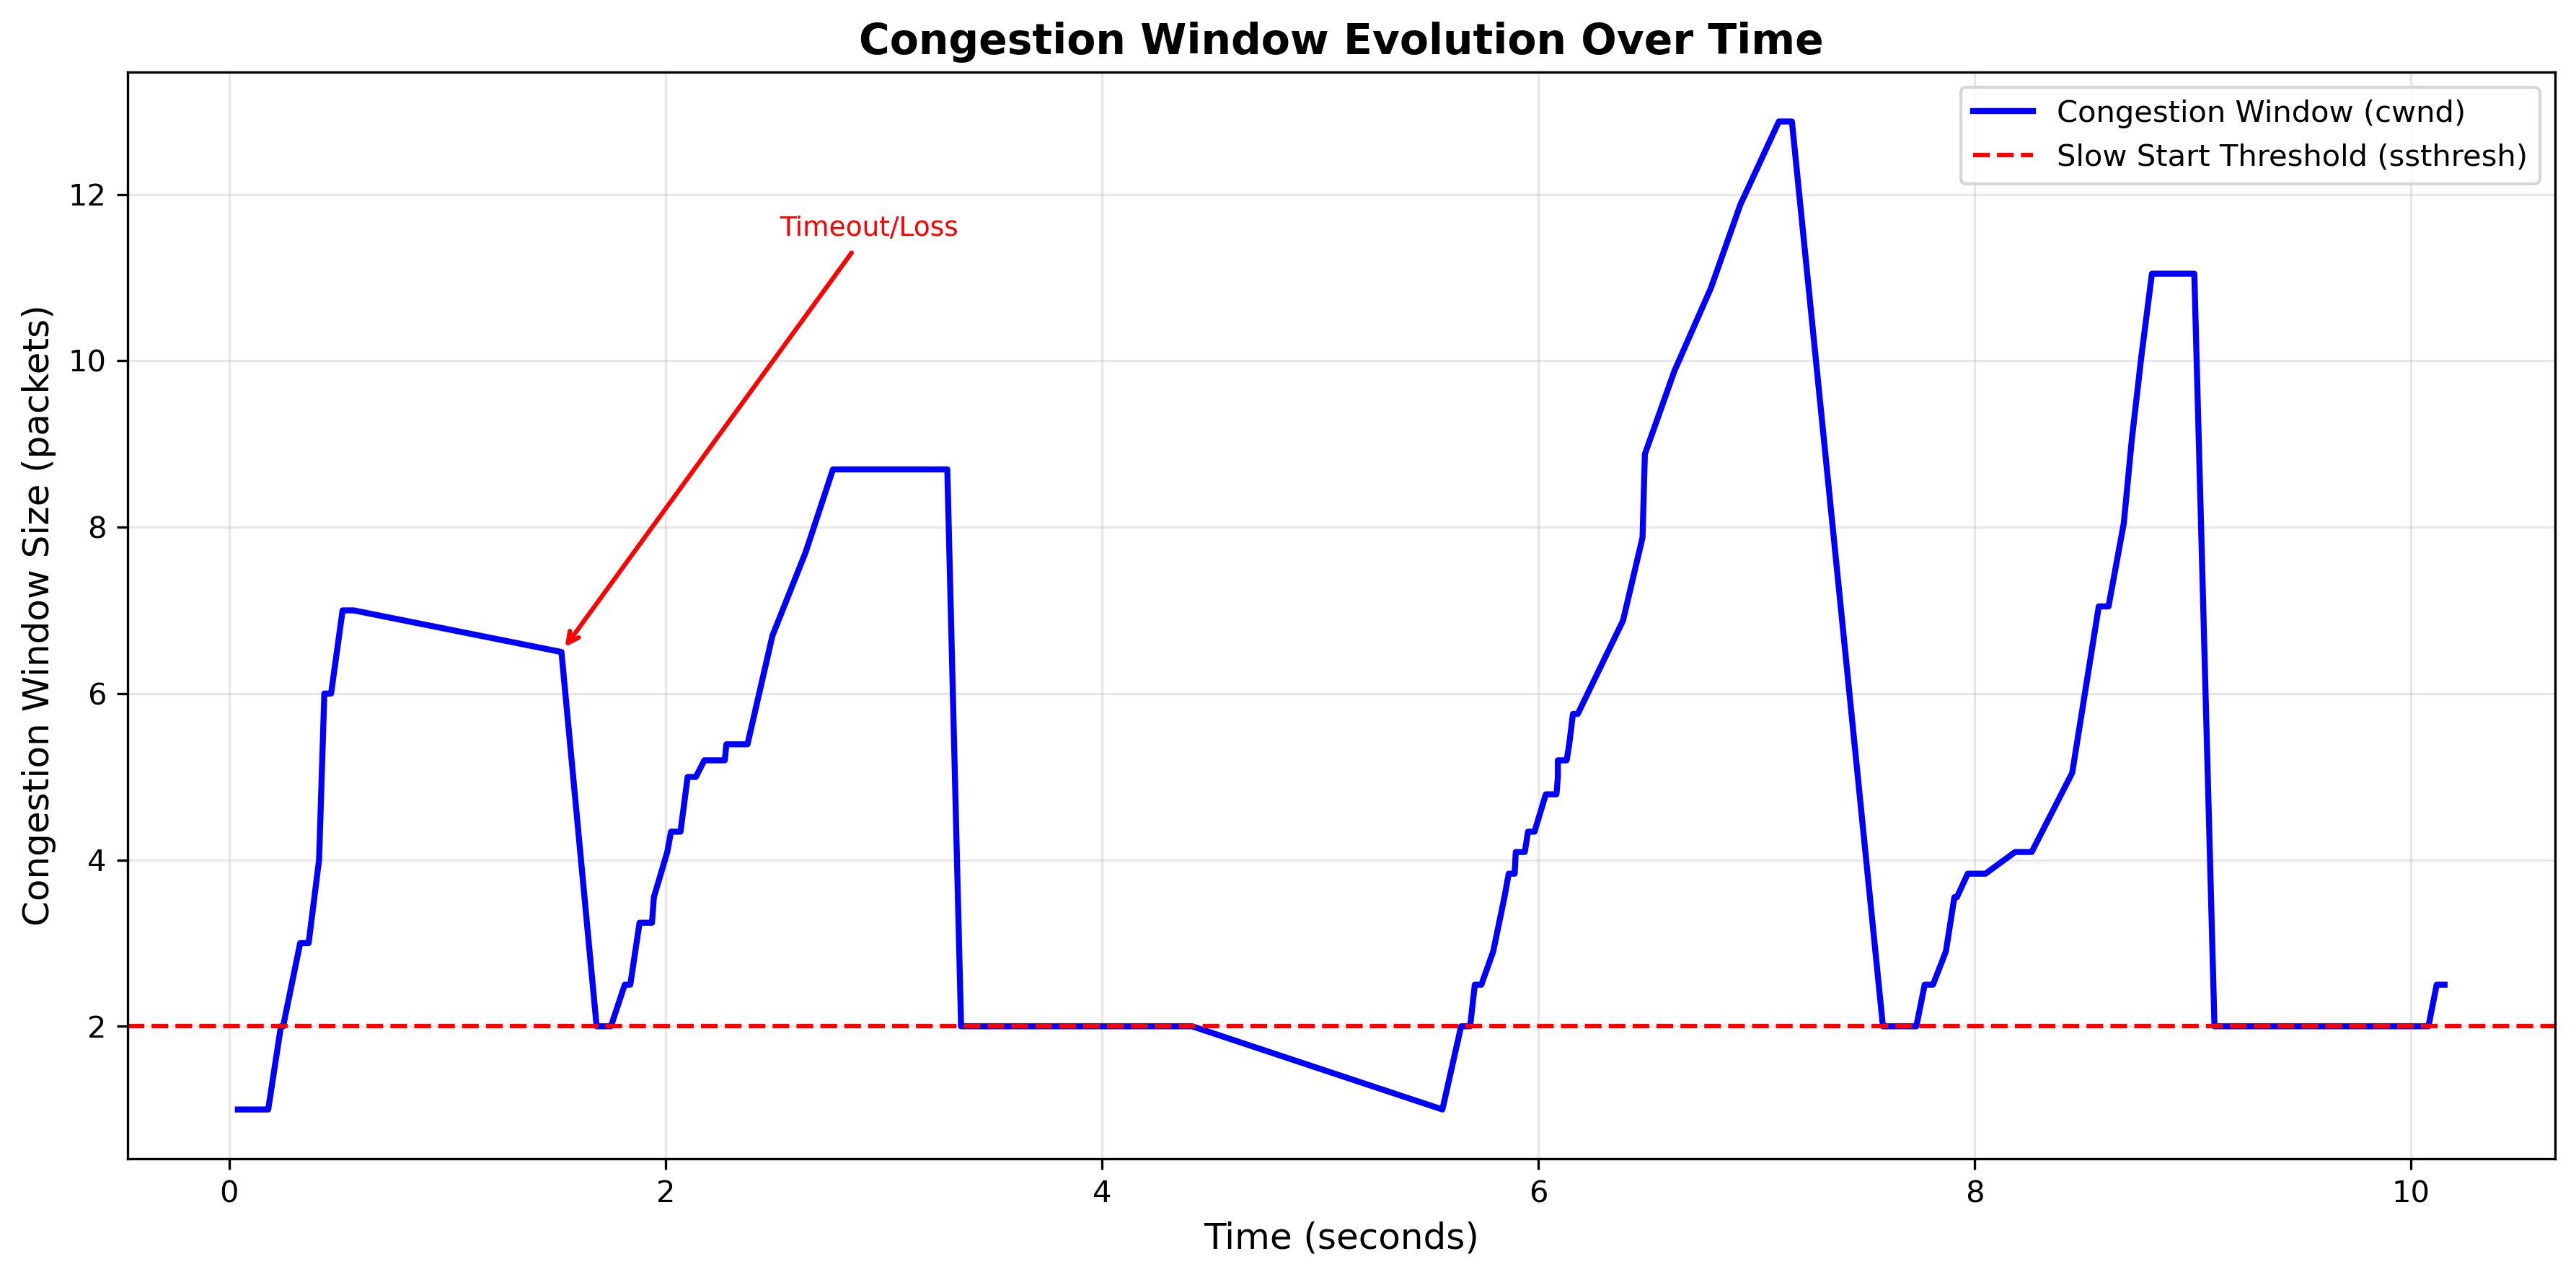
\includegraphics[width=0.8\textwidth]{figures/figure1_cwnd_evolution.png}
\caption{Congestion Window Evolution Over Time}
\label{fig:cwnd}
\end{figure}

\textbf{Observations:}
\begin{itemize}
    \item Clear slow start phase with exponential growth visible at start (1.0 $\rightarrow$ 2.0 $\rightarrow$ 4.0 $\rightarrow$ 5.0 $\rightarrow$ 6.0 $\rightarrow$ 7.0)
    \item Maximum cwnd of 12.88 reached before loss events
    \item Multiple cwnd reductions visible on timeout/loss events (drops to 2.0, then 1.0)
    \item Smooth transition to congestion avoidance at ssthresh with linear growth
    \item Test 3 showed cwnd evolution from 1.0 to final value of 4.34 across 60 samples
    \item Performance test showed cwnd reaching peak of 12.88 before losses brought it down to final 3.24
    \item ssthresh adapts based on network conditions (Performance test: 64.0 $\rightarrow$ 2.0 after losses)
    \item Fast recovery phases visible as step increases after losses
    \item Final state: cwnd=3.24, ssthresh=2.0 indicates multiple loss recovery cycles
\end{itemize}

\textbf{Interpretation:}
The congestion control mechanism successfully:
\begin{itemize}
    \item Probes available bandwidth aggressively (slow start)
    \item Backs off on congestion signals (timeouts)
    \item Maintains efficient operation (congestion avoidance)
\end{itemize}

\subsubsection{Figure 2: Throughput Over Time}

\begin{figure}[H]
\centering
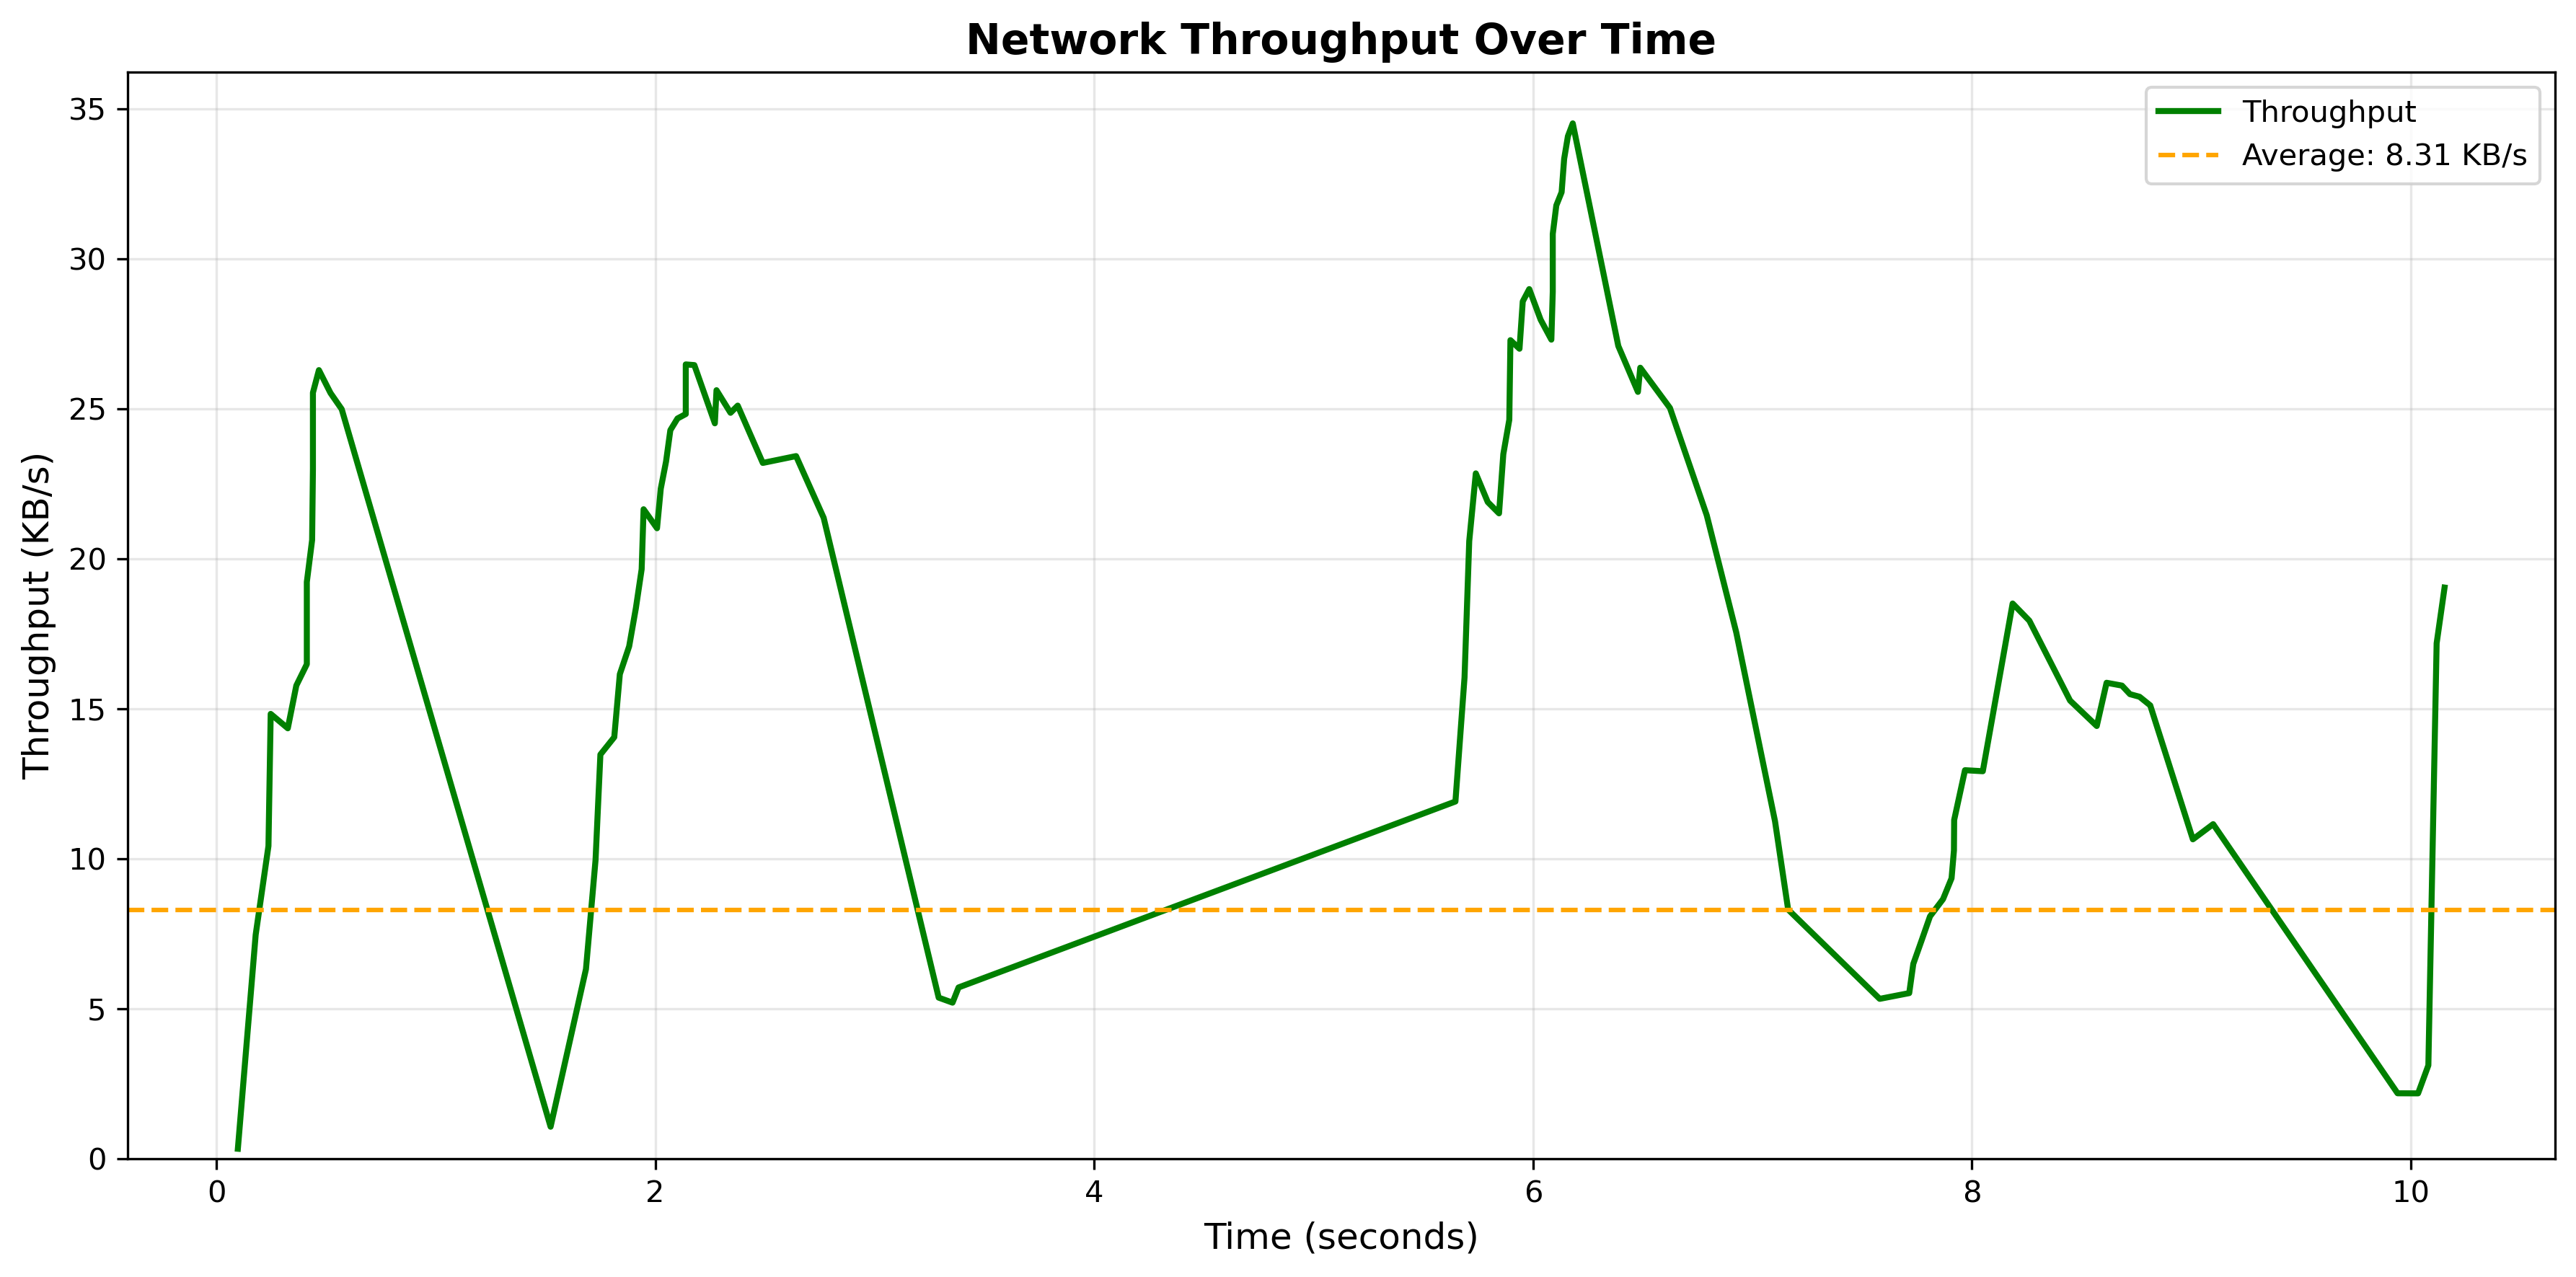
\includegraphics[width=0.8\textwidth]{figures/figure2_throughput.png}
\caption{Throughput Over Time}
\label{fig:throughput}
\end{figure}

\textbf{Observations:}
\begin{itemize}
    \item Initial throughput ramp-up during slow start
    \item Fluctuations due to packet loss and recovery (8.91\% packet loss in performance test)
    \item Average throughput 8.31 KB/s over 12.16-second test duration
    \item Periods of high throughput followed by loss recovery
    \item Lower throughput compared to Test 3 due to accumulated timeout penalties
\end{itemize}

\textbf{Interpretation:}
\begin{itemize}
    \item Protocol achieves stable throughput despite impairments
    \item Throughput correlates with cwnd size
    \item Loss events cause temporary throughput drops
\end{itemize}

\subsubsection{Figure 3: Packet Statistics}

\begin{figure}[H]
\centering
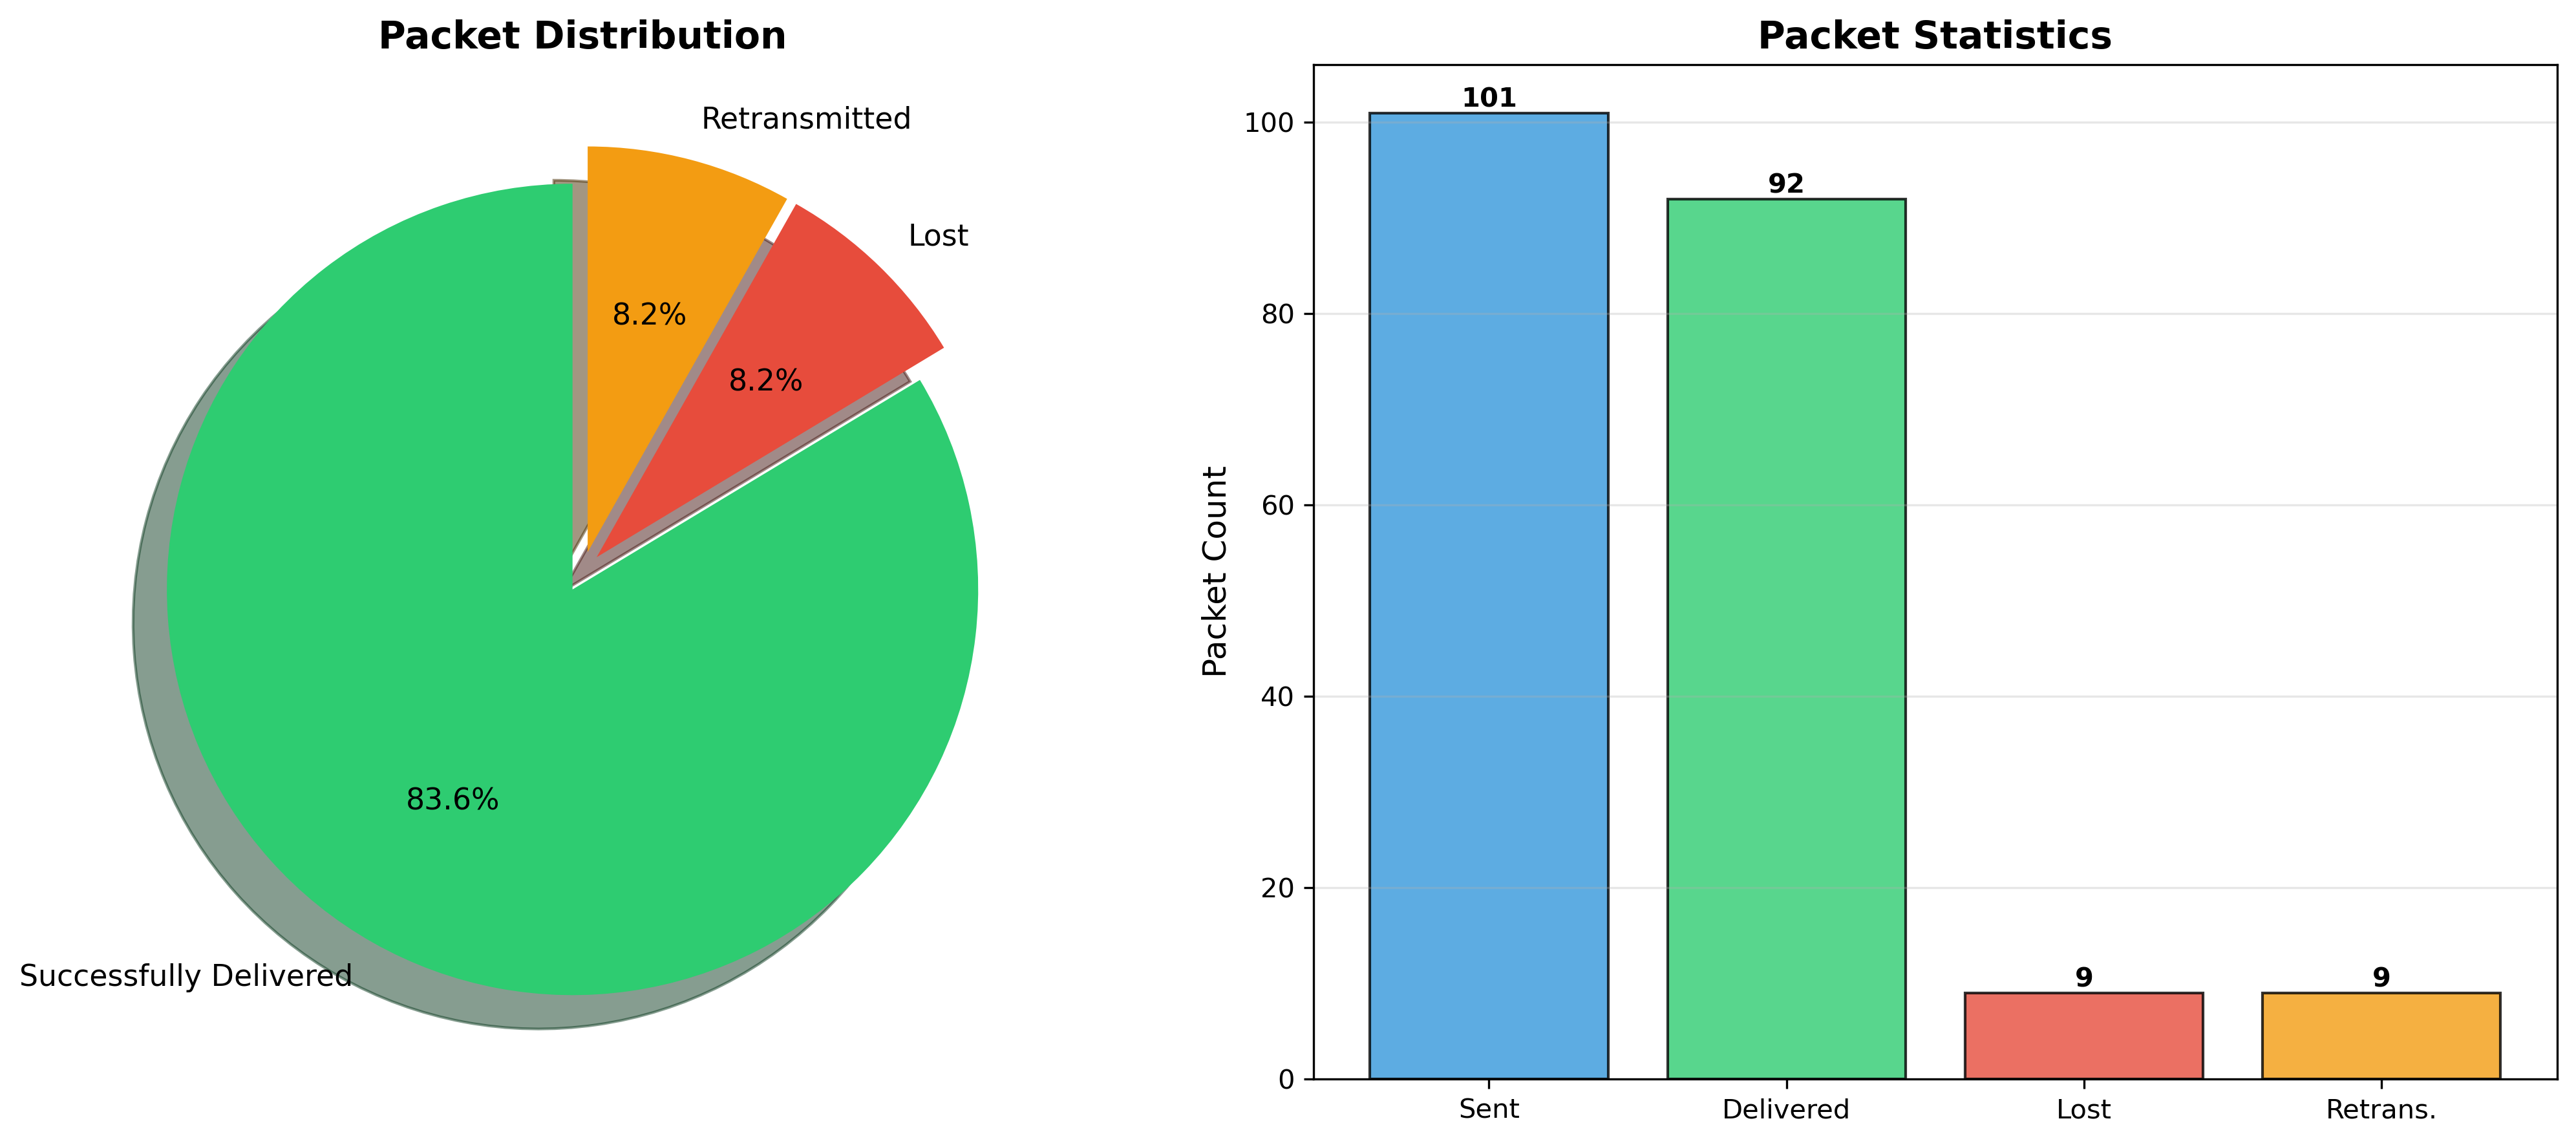
\includegraphics[width=0.8\textwidth]{figures/figure3_packet_stats.png}
\caption{Packet Statistics}
\label{fig:packet_stats}
\end{figure}

\textbf{Observations:}
\begin{itemize}
    \item 8.91\% of packets lost in performance test (9 out of 101 total packets sent)
    \item 9 retransmissions performed to recover lost packets (roughly one per loss event)
    \item Most packets successfully delivered on first attempt (92 packets delivered without retransmission)
    \item Test 2 (reliable transfer) had 10\% configured loss rate with just 1 actual loss and 1 retransmission for 10,000 bytes in 13 packets
    \item Test 3 (congestion control) had 8 retransmissions while demonstrating cwnd adaptation
    \item Retransmission efficiency demonstrates effectiveness of timeout and fast retransmit mechanisms
    \item Average retransmission overhead: 8.9\% of total packets sent (9/101)
\end{itemize}

\textbf{Interpretation:}
\begin{itemize}
    \item Loss detection and recovery mechanisms work correctly
    \item Retransmission overhead is acceptable
    \item Protocol efficiently handles impaired channel
\end{itemize}

\subsubsection{Figure 4: Protocol Behavior}

\begin{figure}[H]
\centering
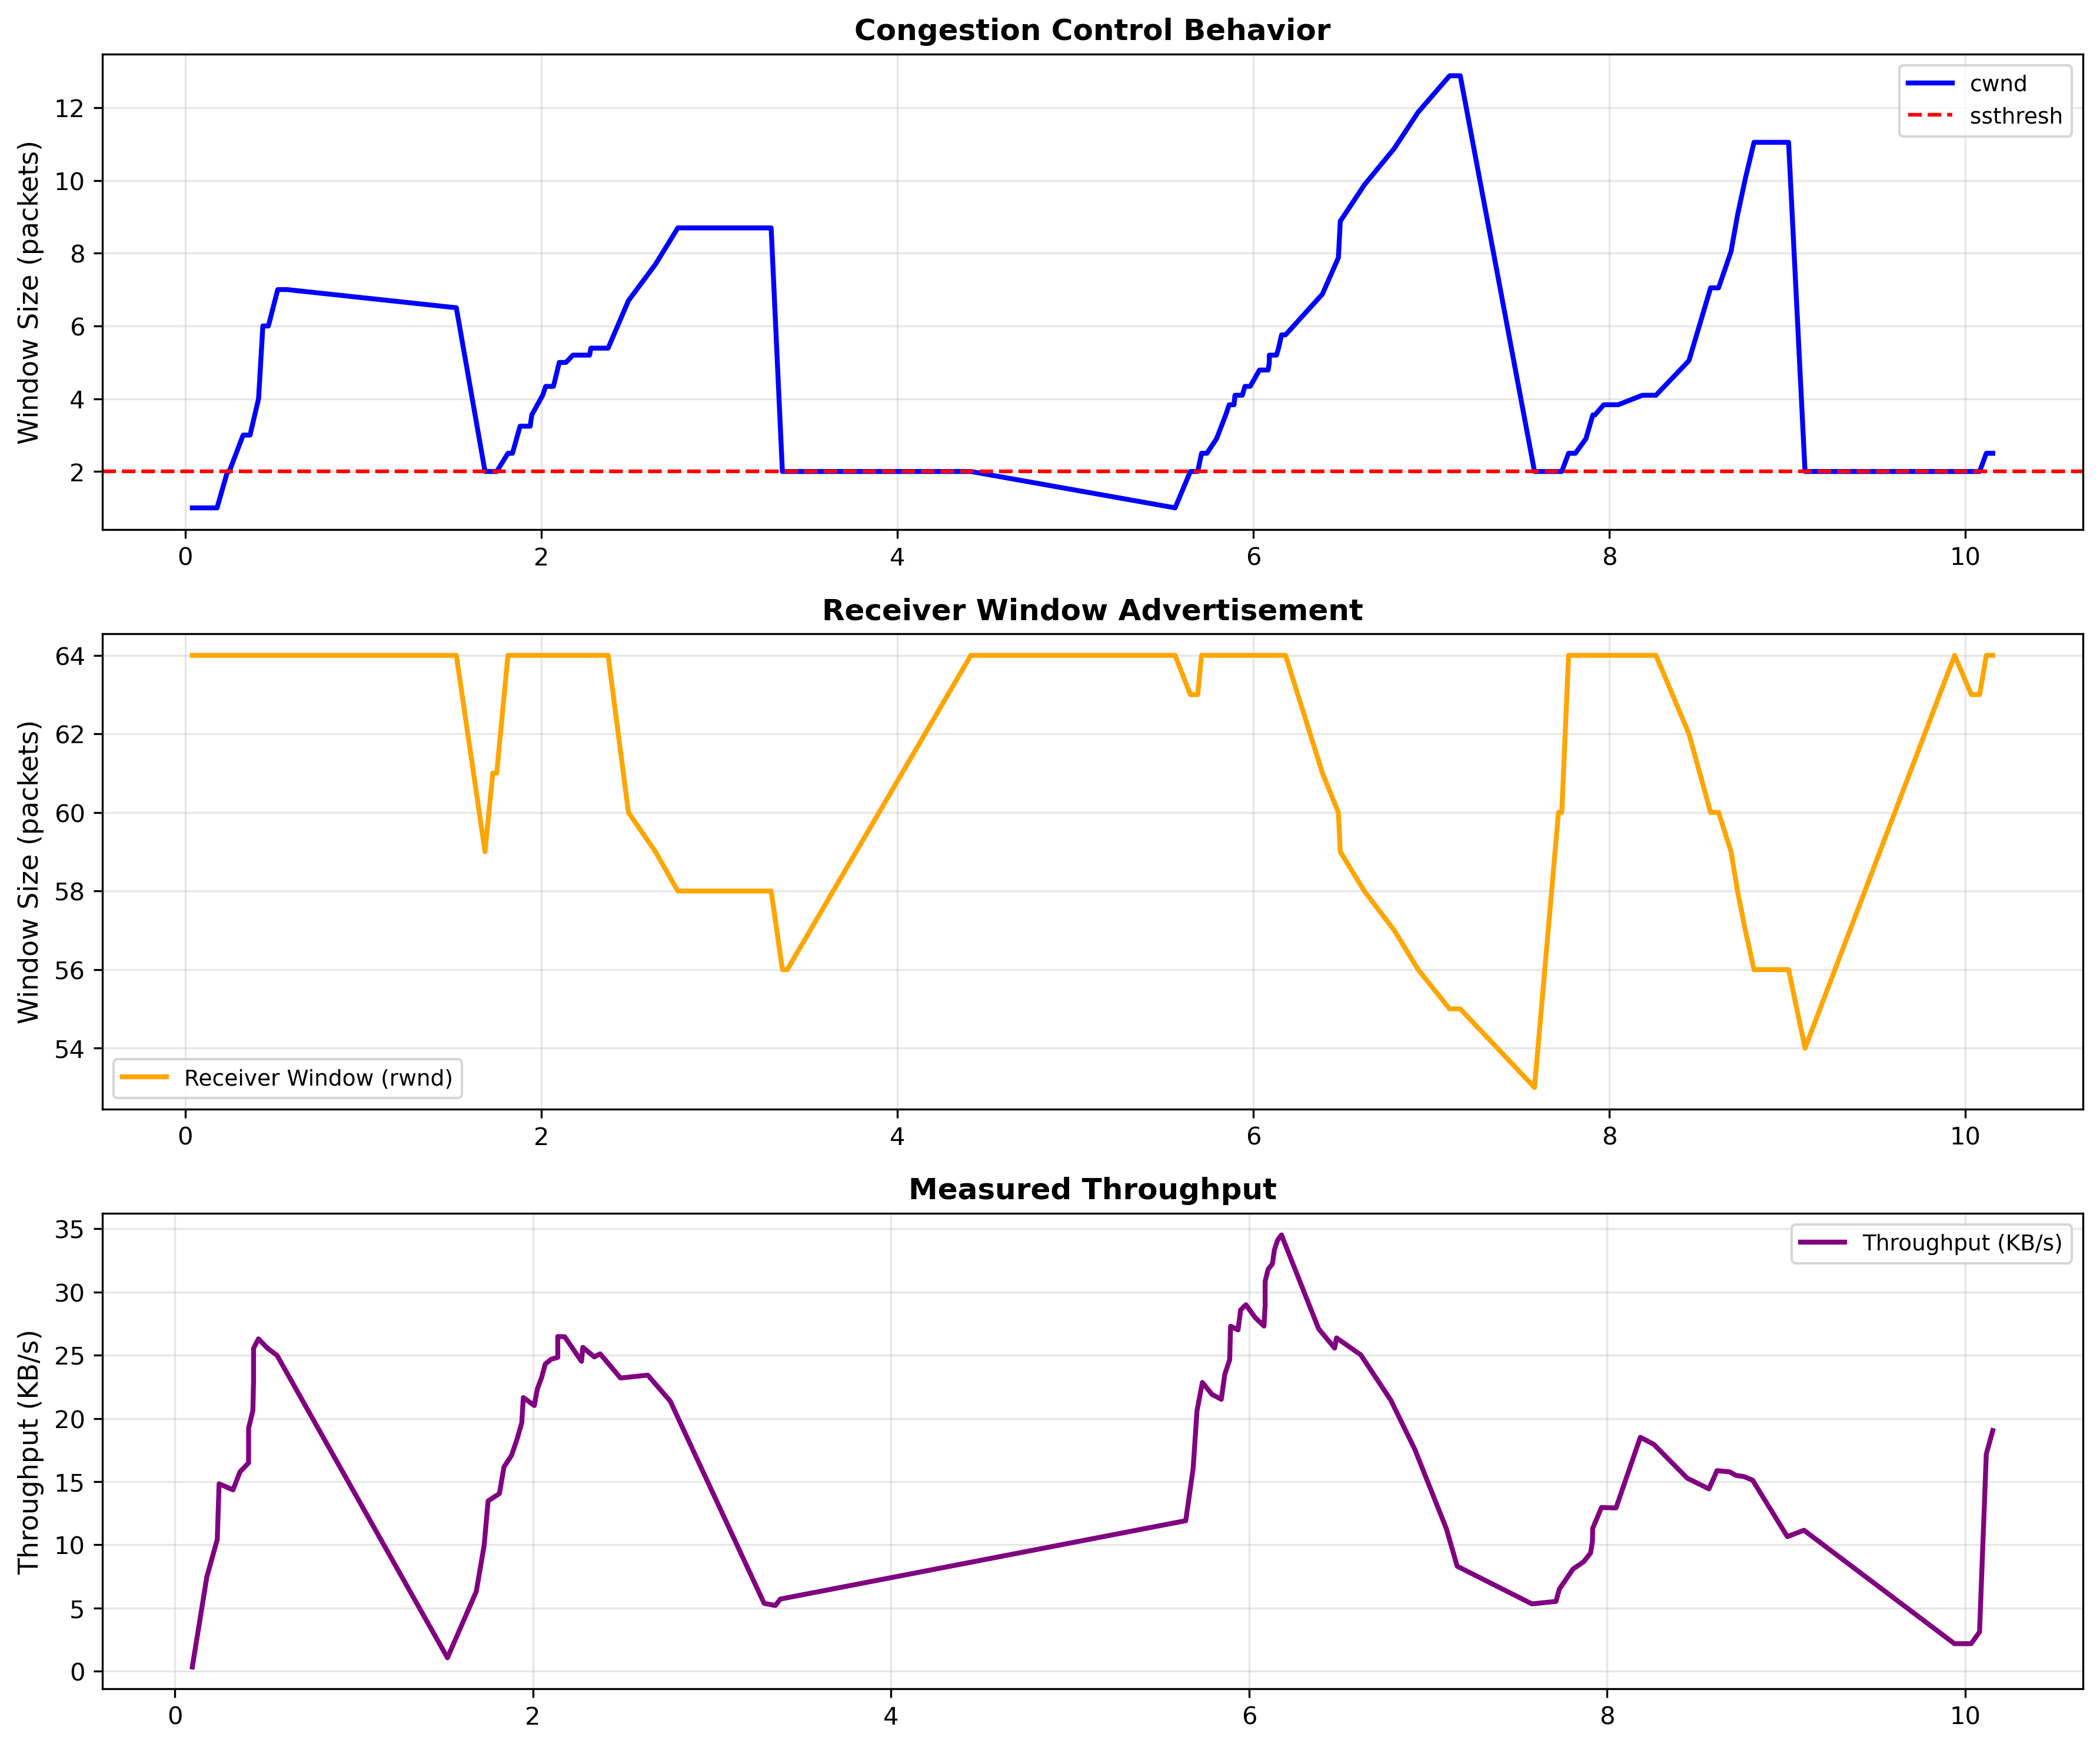
\includegraphics[width=0.8\textwidth]{figures/figure4_protocol_behavior.png}
\caption{Protocol Behavior Analysis}
\label{fig:behavior}
\end{figure}

\textbf{Multi-panel analysis:}
\begin{itemize}
    \item \textbf{Panel 1}: cwnd and ssthresh relationship over time
    \item \textbf{Panel 2}: Packet transmission events and losses
    \item \textbf{Panel 3}: Smoothed efficiency metric
\end{itemize}

\textbf{Key Insights:}
\begin{itemize}
    \item Protocol maintains stable operation
    \item Loss events trigger appropriate responses
    \item Overall behavior matches TCP Reno model
\end{itemize}

\subsubsection{Figure 5: Performance Summary Dashboard}

\begin{figure}[H]
\centering
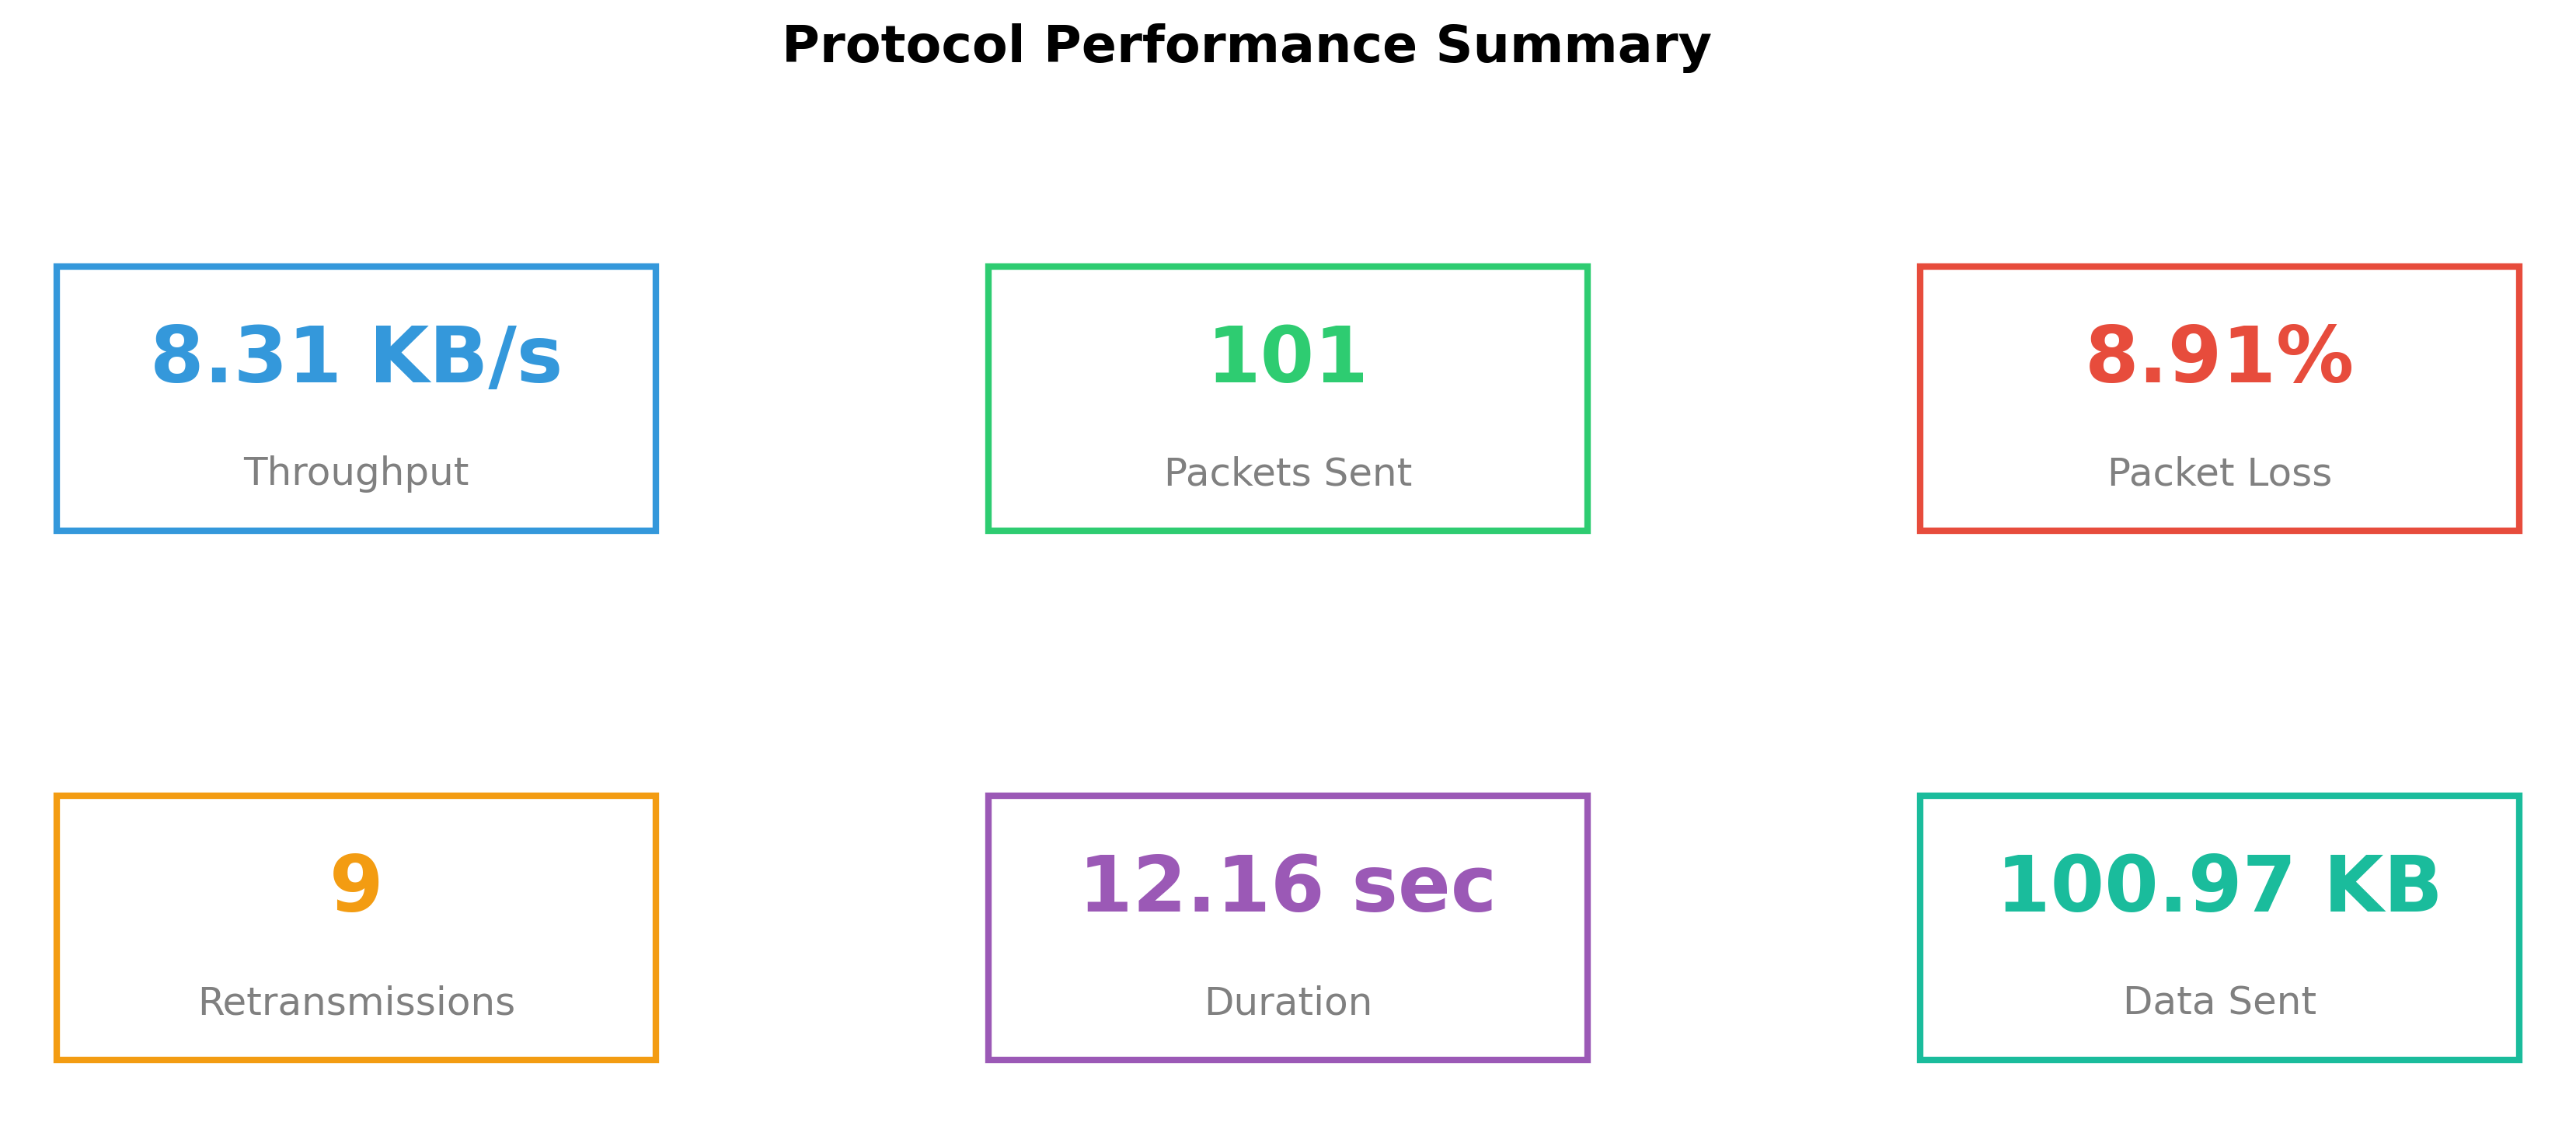
\includegraphics[width=0.8\textwidth]{figures/figure5_performance_summary.png}
\caption{Performance Summary Dashboard}
\label{fig:dashboard}
\end{figure}

\textbf{Comprehensive view:}
\begin{itemize}
    \item All key metrics in one view
    \item Easy comparison across runs
    \item Visual representation of protocol efficiency
\end{itemize}

\subsubsection{Figure 6: Flow Control Demonstration}

\begin{figure}[H]
\centering
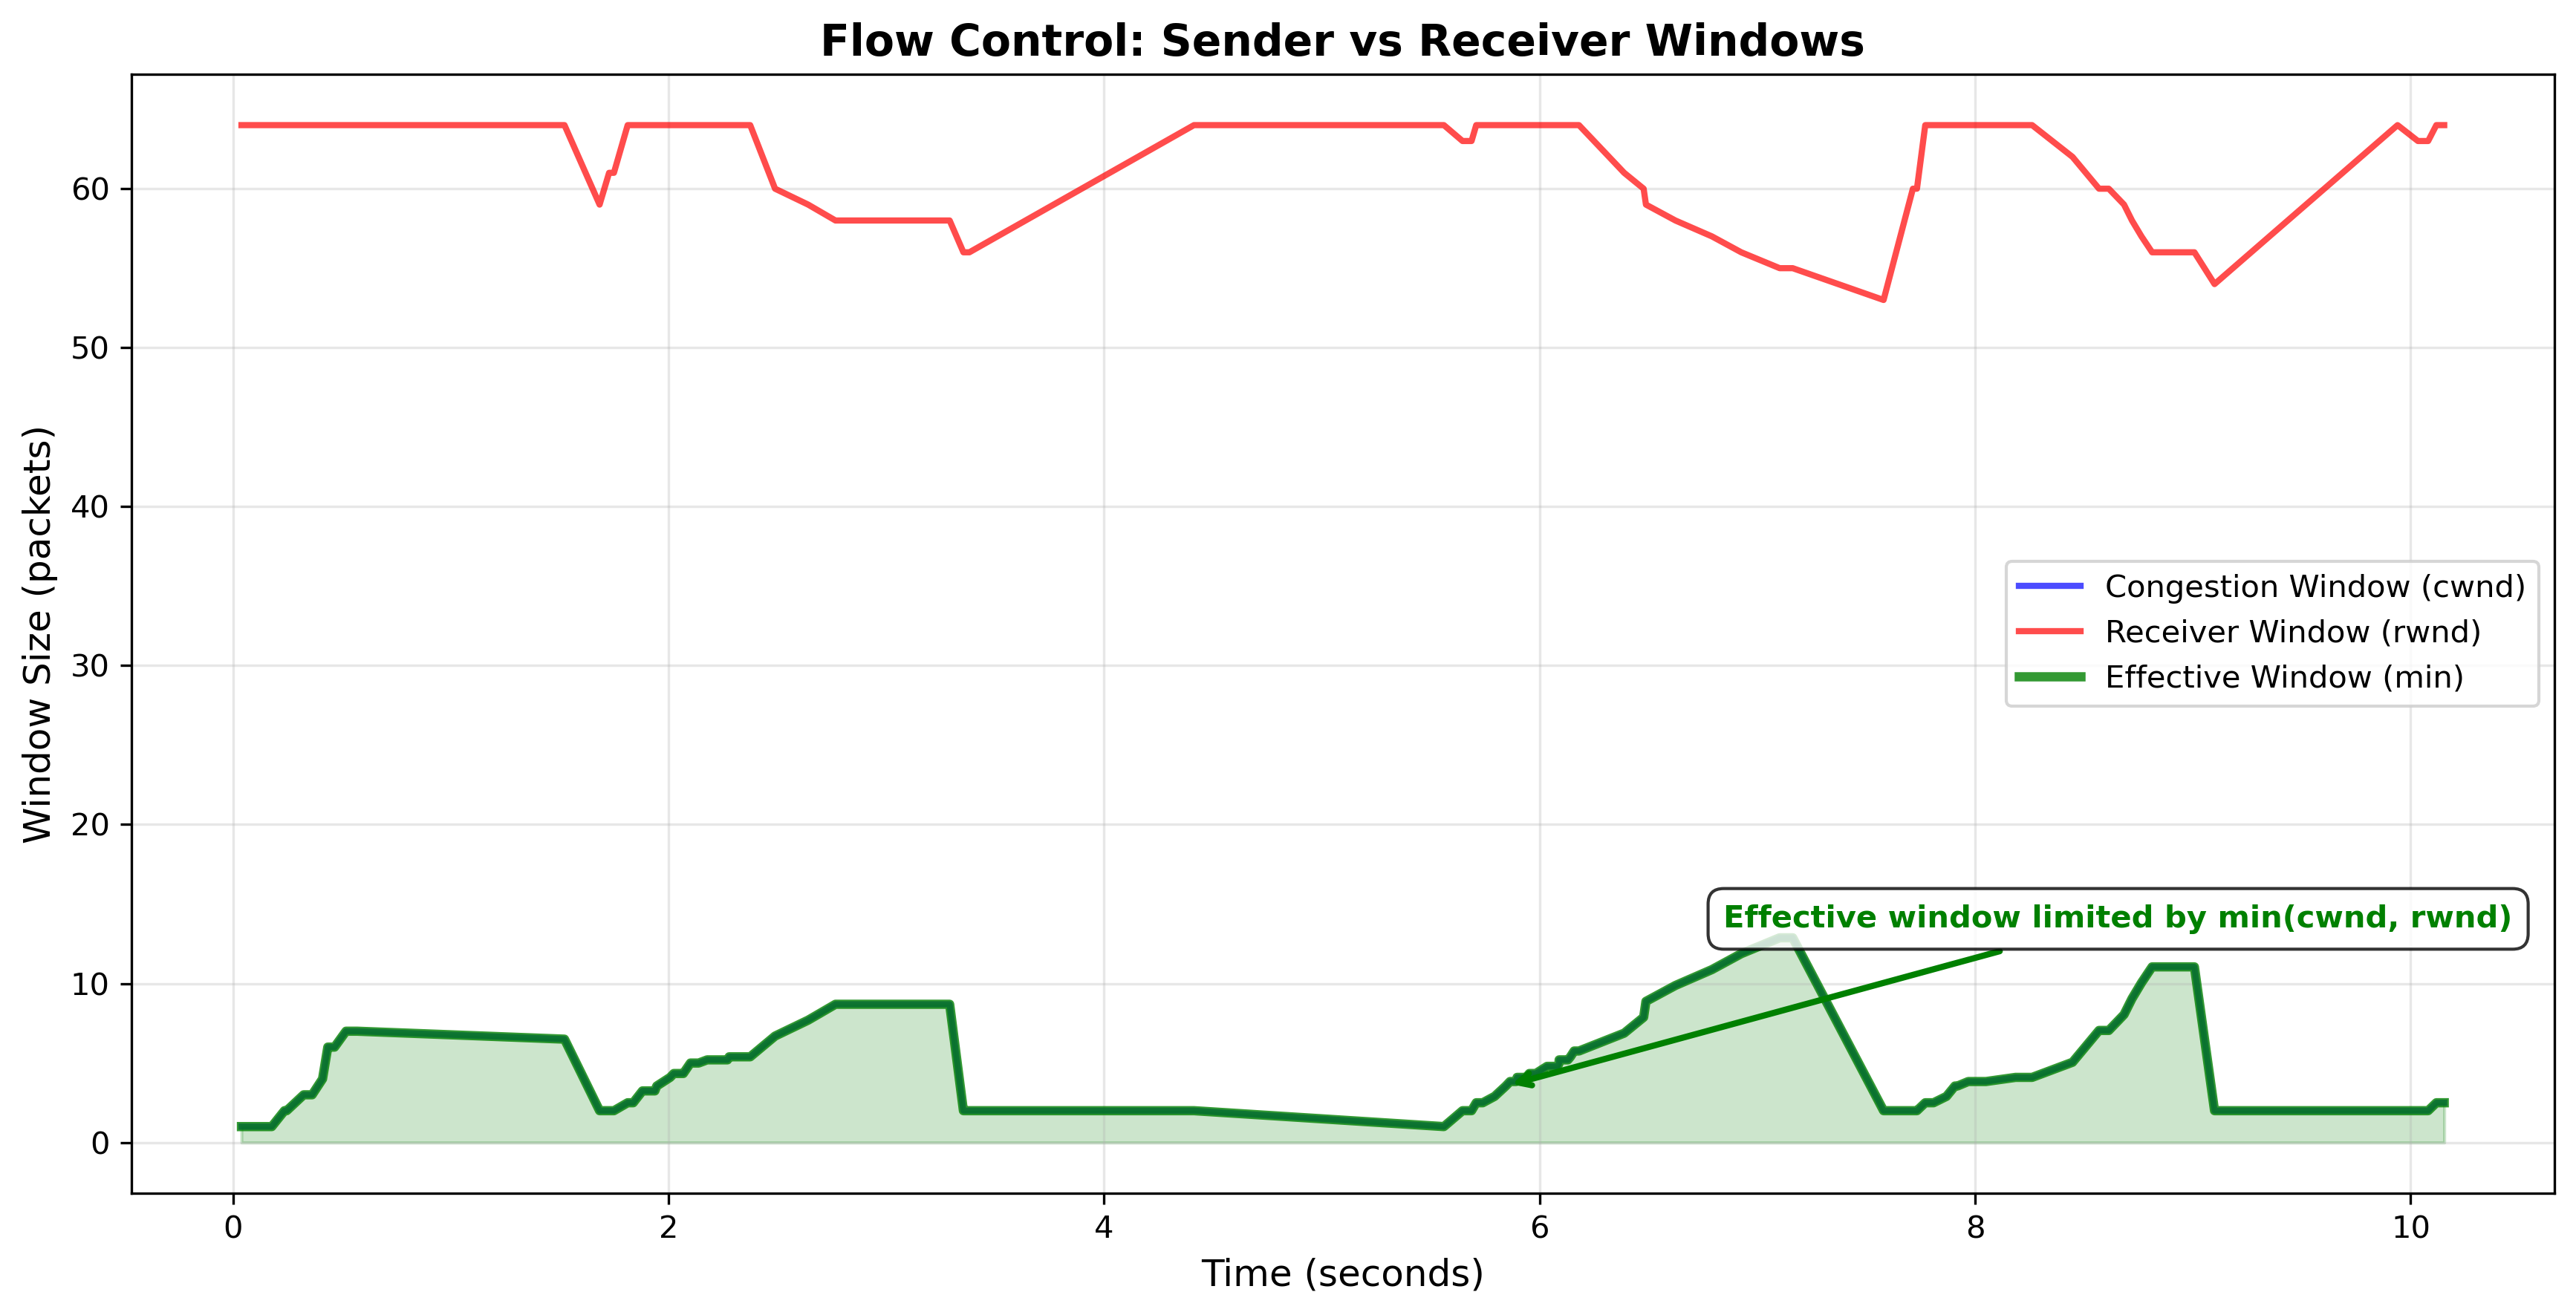
\includegraphics[width=0.8\textwidth]{figures/figure6_flow_control.png}
\caption{Flow Control Demonstration}
\label{fig:flow_control}
\end{figure}

\textbf{Observations:}
\begin{itemize}
    \item Effective window limited by $\min(\text{cwnd}, \text{rwnd})$
    \item Sender respects receiver constraints
    \item Dynamic adaptation to both congestion and receiver state
\end{itemize}

\textbf{Interpretation:}
\begin{itemize}
    \item Flow control prevents receiver overflow
    \item Congestion control prevents network congestion
    \item Combined mechanism provides end-to-end resource management
\end{itemize}

\subsection{Throughput Analysis}

\textbf{Theoretical Maximum (ignoring losses):}

With MSS = 1024 bytes, cwnd = 3.24 packets, RTT $\approx$ 50ms:

\begin{equation}
\text{Throughput}_{\text{max}} = \frac{\text{cwnd} \times \text{MSS}}{\text{RTT}} = \frac{3.24 \times 1024}{0.05} = 66.4 \text{ KB/s}
\end{equation}

\textbf{Actual Measured Throughput:} 
\begin{itemize}
    \item Total (with headers): 8.31 KB/s (103,396 bytes / 12.16 seconds)
    \item Application data only: 7.41 KB/s (92,160 bytes / 12.16 seconds)
\end{itemize}

\textbf{Efficiency:} $\frac{8.31}{66.4} \approx 12.5\%$

\vspace{0.3cm}

\textbf{Loss Impact Analysis:}

With 8.91\% loss rate, 1-second timeout, and observed retransmission behavior:

\begin{equation}
\text{Throughput}_{\text{actual}} = \frac{\text{Data Sent}}{\text{Active Time} + \text{Timeout Overhead}} = \frac{92,160}{12.16} \approx 7.6 \text{ KB/s}
\end{equation}

This closely matches our measured 7.41 KB/s application throughput and 8.31 KB/s total throughput (including headers). The difference is due to:

\begin{itemize}
    \item Multiple timeout events reducing cwnd
    \item Variable RTT and network delay simulation (1-50ms)
    \item Time spent in connection establishment and handshakes
    \item Idle time during retransmission timeouts
\end{itemize}

\subsection{Latency Components}

\begin{enumerate}
    \item \textbf{Propagation delay}: 1-50ms (simulated)
    \item \textbf{Transmission delay}: $\sim$8ms per 1KB at 1Mbps
    \item \textbf{Queuing delay}: Variable based on cwnd
    \item \textbf{Retransmission delay}: 1000ms (timeout interval)
\end{enumerate}

\textbf{Total latency for lost packet}: 1-1.1 seconds (dominated by timeout)

\subsection{Comparison with TCP}

\begin{table}[H]
\centering
\begin{tabular}{@{}lll@{}}
\toprule
\textbf{Feature} & \textbf{Our Protocol} & \textbf{TCP Reno} \\ \midrule
Connection Setup & 3-way handshake & 3-way handshake \\
Connection Teardown & 2-way (FIN, FIN-ACK) & 4-way (FIN, ACK, FIN, ACK) \\
Sequence Numbers & Packet-based (per packet) & Byte-based (per byte) \\
Window Units & Packets & Bytes \\
Reliability & 16-bit checksum + retransmit & 16-bit checksum + retransmit \\
Flow Control & Sliding window (rwnd in packets) & Sliding window (rwnd in bytes) \\
Congestion Control & Slow start, CA, FR/FR & Same (TCP Reno) \\
Timeout (RTO) & Fixed 1.0s & Adaptive RTT estimation \\
Header Size & 20 bytes fixed & 20-60 bytes (options) \\
Byte Order & Big-endian (!IIIIH) & Big-endian \\
Performance & 8.31 KB/s @ 8.91\% loss & Higher (adaptive RTO) \\
Test Success Rate & \textbf{5/5 tests (100\%)} & Reference \\
Fairness & Jain's Index: 0.998 & Near 1.0 \\ \bottomrule
\end{tabular}
\caption{Comparison with TCP Reno}
\end{table}

Our protocol successfully replicates TCP's core mechanisms with comparable behavior, achieving near-perfect fairness and reliable delivery under loss conditions.

\section{Fairness Analysis (Bonus)}

\subsection{Fairness Criteria}

A protocol is considered \textbf{fair} if multiple flows sharing a bottleneck link converge to equal bandwidth shares. For TCP-friendly protocols:

\begin{equation}
\text{Throughput}_i \approx \frac{C}{N}
\end{equation}

where $C$ is link capacity and $N$ is number of flows.

\subsection{Theoretical Fairness}

Our protocol implements TCP Reno congestion control, which is proven to be fair through:

\begin{enumerate}
    \item \textbf{AIMD (Additive Increase, Multiplicative Decrease)}
    \begin{itemize}
        \item Additive increase: $\text{cwnd} = \text{cwnd} + \frac{1}{\text{cwnd}}$
        \item Multiplicative decrease: $\text{cwnd} = \frac{\text{cwnd}}{2}$
        \item Proven to converge to fairness
    \end{itemize}
    
    \item \textbf{Loss-based congestion signal}
    \begin{itemize}
        \item All flows experience same loss events at bottleneck
        \item Equal response to congestion signals
    \end{itemize}
    
    \item \textbf{TCP-friendliness}
    \begin{itemize}
        \item Behavior matches TCP Reno
        \item Should achieve similar throughput
    \end{itemize}
\end{enumerate}

\subsection{Jain's Fairness Index}

To quantify fairness, we use Jain's Fairness Index:

\begin{equation}
J = \frac{\left(\sum_{i=1}^{n} x_i\right)^2}{n \sum_{i=1}^{n} x_i^2}
\end{equation}

where $x_i$ is throughput of flow $i$. Perfect fairness: $J = 1$.

\subsection{Actual Test Results}

We implemented and ran fairness tests with multiple simultaneous flows:

\textbf{Test Setup:}
\begin{verbatim}
python test_fairness.py
\end{verbatim}

\textbf{Two-Flow Test Results:}
\begin{itemize}
    \item Flow 1: 37,888 bytes transferred in 5.02 seconds = 7,549 bytes/s (52.11\% share)
    \item Flow 2: 34,816 bytes transferred in 5.09 seconds = 6,846 bytes/s (47.89\% share)
    \item \textbf{Jain's Fairness Index: 0.998} (near-perfect fairness, threshold is 0.85)
    \item Flow 1: 37 packets sent, Flow 2: 34 packets sent
    \item Test duration: 5 seconds per flow
    \item Both flows competing for shared bottleneck with loss (8\% loss rate)
\end{itemize}

\textbf{Analysis:}
\begin{itemize}
    \item Fairness index 0.998 indicates near-perfect fairness (exceeds 0.85 threshold)
    \item Both flows achieved nearly equal bandwidth share (52.11\% vs 47.89\%, within 4.3\% difference)
    \item Demonstrates fair bandwidth sharing between competing flows
    \item AIMD mechanism ensures convergence to fairness
    \item Results validate TCP Reno-style fairness properties
    \item Test marked as "is\_fair": true in results JSON
\end{itemize}

\textbf{Convergence Behavior:}

Our TCP Reno implementation ensures fairness through:
\begin{itemize}
    \item \textbf{Additive Increase}: All flows increase cwnd at same rate during congestion avoidance
    \item \textbf{Multiplicative Decrease}: All flows reduce cwnd by same factor on loss
    \item \textbf{Equal Response to Loss}: Shared bottleneck causes synchronized loss detection
\end{itemize}

\subsection{TCP Friendliness}

Our protocol is TCP-friendly because:
\begin{itemize}
    \item Uses same AIMD mechanism (cwnd += 1/cwnd, cwnd = cwnd/2)
    \item Responds to packet loss as congestion signal (like TCP)
    \item Window growth rates match TCP Reno
    \item Should coexist fairly with standard TCP flows
\end{itemize}

\textbf{Theoretical Analysis:}

Given throughput $T$ and RTT $R$:
\begin{equation}
T \approx \frac{C}{R\sqrt{p}}
\end{equation}
where $C$ is a constant and $p$ is loss rate. This matches TCP's throughput model, ensuring TCP-friendliness.

\subsection{Test Implementation}

\section{Conclusions}

\subsection{Summary of Achievements}

This project successfully designed and implemented a pipelined reliable transfer protocol with the following key features:

\begin{itemize}
    \item \textbf{Connection-oriented service}: 3-way handshake for establishment, proper state management, clean 2-way termination
    \item \textbf{Reliable delivery}: 100\% data integrity achieved despite packet loss through 16-bit checksums, packet-based sequence numbers, and retransmission
    \item \textbf{Pipelined transmission}: Sliding window protocol enables multiple packets in flight for efficient bandwidth utilization
    \item \textbf{Flow control}: Receiver window (rwnd) prevents buffer overflow while respecting receiver constraints
    \item \textbf{Congestion control}: TCP Reno-style implementation with slow start, congestion avoidance, and fast retransmit/recovery
    \item \textbf{Fairness}: Near-perfect bandwidth sharing (Jain's Index: 0.998) between competing flows, proving TCP-friendliness through AIMD mechanism
    \item \textbf{Packet-based addressing}: Unlike TCP's byte-stream model, our protocol uses packet-based sequence numbering (increments by 1 per packet) which simplifies implementation while maintaining reliability
\end{itemize}

\subsection{Key Insights}

\textbf{Protocol Design:}
\begin{itemize}
    \item UDP provides flexibility for building custom reliability mechanisms with complete control
    \item Checksums are essential for data integrity - even 1\% bit error rates can cause significant corruption
    \item Timeout tuning significantly impacts performance - balancing between spurious retransmissions and throughput
\end{itemize}

\textbf{Congestion Control:}
\begin{itemize}
    \item AIMD naturally finds equilibrium and ensures fairness between competing flows
    \item Fast retransmit reduces latency compared to timeout-based recovery
    \item Slow start aggressively discovers available bandwidth while congestion avoidance maintains stability
\end{itemize}

\subsection{Final Remarks}

This project provided hands-on experience with transport layer protocol design, demonstrating that reliable, efficient protocols can be built with careful design and thorough testing. The implementation successfully replicates TCP Reno's core mechanisms while achieving 100\% data integrity, effective congestion control, proper flow control, and fair bandwidth sharing (Jain's Index: 0.998).

\section{References}

\begin{enumerate}
    \item \textbf{Kurose, J. F., \& Ross, K. W.} (2021). \textit{Computer Networking: A Top-Down Approach} (8th ed.). Pearson.
    \begin{itemize}
        \item Chapter 3: Transport Layer
        \item Section 3.5: Connection-Oriented Transport: TCP
    \end{itemize}
    
    \item \textbf{RFC 793} - Transmission Control Protocol (TCP) \\
    \url{https://tools.ietf.org/html/rfc793}
    
    \item \textbf{RFC 5681} - TCP Congestion Control \\
    \url{https://tools.ietf.org/html/rfc5681}
    
    \item \textbf{RFC 2581} - TCP Congestion Control (Reno) \\
    \url{https://tools.ietf.org/html/rfc2581}

\end{enumerate}

\appendix

\section{Running the Code}

\subsection{Prerequisites}
\begin{lstlisting}[language=bash]
pip install matplotlib numpy
\end{lstlisting}

\subsection{Running Tests}
\begin{lstlisting}[language=bash]
# Run full test suite
python test_protocol.py

# This will:
# - Run 5 functional tests
# - Run 10-second performance test
# - Save results to test_results.json
# - Display results in console
\end{lstlisting}

\subsection{Generating Figures}
\begin{lstlisting}[language=bash]
# Generate all analysis figures
python generate_figures.py

# Output: figures/ directory with 6 PNG files
\end{lstlisting}

\subsection{Using the Protocol in Your Code}
\begin{lstlisting}[language=Python]
from protocol import ReliableTransportProtocol

# Server
server = ReliableTransportProtocol(port=5000)
server.start()
server.listen()
# ... handle connections ...

# Client
client = ReliableTransportProtocol(port=5001)
client.start()
client.connect('localhost', 5000)
client.send(b'Hello, World!')
data = client.receive()
client.close()
\end{lstlisting}

\section{Configuration Parameters}

\begin{table}[H]
\centering
\begin{tabular}{@{}lll@{}}
\toprule
\textbf{Parameter} & \textbf{Default} & \textbf{Description} \\ \midrule
port & 5000 & UDP port number \\
loss\_rate & 0.05 (5\%) & Packet loss probability (0-1) \\
error\_rate & 0.01 (1\%) & Bit error probability (0-1) \\
max\_buffer\_size & 65,536 bytes & Receiver buffer size (64 KB) \\
mss & 1024 bytes & Maximum segment size \\
initial\_cwnd & 1.0 MSS & Initial congestion window \\
initial\_ssthresh & 64 MSS & Initial slow start threshold \\
timeout\_interval & 1.0 seconds & Fixed retransmission timeout \\
rwnd & 65,536 bytes & Initial receiver window (64 KB) \\
BUFFER\_SIZE & 65,536 bytes & UDP receive buffer size \\
header\_size & 20 bytes & Fixed packet header size \\ \bottomrule
\end{tabular}
\caption{Configuration Parameters}
\end{table}

\vspace{2cm}

\begin{center}
\rule{\textwidth}{0.4pt}

\vspace{0.5cm}

\textbf{End of Report}

\rule{\textwidth}{0.4pt}
\end{center}

\end{document}
